\begin{frame}
	\frametitle{Double-Ended Queues}

	\begin{center}
		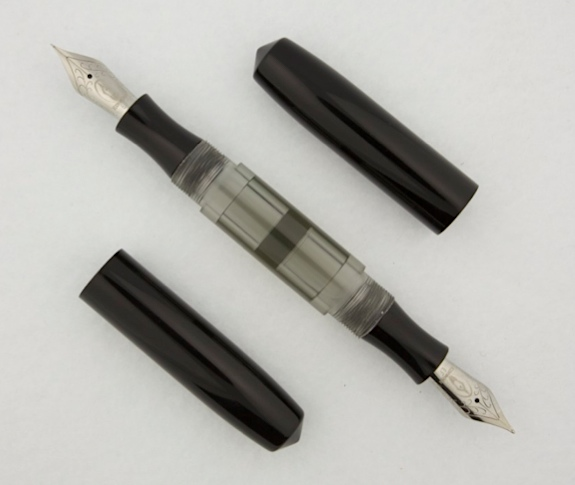
\includegraphics[width=0.5\textwidth]{figures/de.jpg}\\
		\hspace*{15pt}\hbox{\scriptsize Image By:\thinspace{\itshape Chris Lott}}
		% https://www.flickr.com/photos/fncll/9824392125
	\end{center}
\end{frame}

\begin{frame}
	\frametitle{Deques}
		\begin{block}{Deques}
			Deques, or Double-Ended Queues, allow both FIFO and LIFO operations in $O(1)$ time.
		\end{block}		
		\pause
		\begin{questionblock}{Hang on...}
			Doesn't that sound familiar?	
		\end{questionblock}
		\pause
		\begin{answerblock}{Back to DLL}
			This is exactly what a DLL offers!
		\end{answerblock}
\end{frame}

\begin{frame}
	\frametitle{\texttt{deque}}
	
	In python we can use a \texttt{deque} called \texttt{d} on which:
	\begin{itemize}
		\item We can \textit{push} with \texttt{d.append}.
		\item We can \textit{pop} with \texttt{d.pop}.
		\item We can \textit{top} with \texttt{d[-1]}
			\pause
		\item We can \textit{enqueue} with \texttt{d.append}.
		\item We can \textit{dequeue} with \texttt{d.popleft}.
		\item We can \textit{peek} with \texttt{d[0]}
			\pause
		\item Oh yeah and if you want, you can also add to the left with \texttt{appendleft}
	\end{itemize}
\end{frame}


